\section{RGB laserový modul}
Jako zdroj laserového paprsku byl využit RGB laserový modul, skládající se~ze řídící desky, tří barevných laserových diod o vlnových délkách 660~nm~(červená), 450~nm~(modrá) a~520~nm~(zelená) a~tří dichroických zrcátek, která slouží ke~spojení paprsků z~diod do~jednoho. Celý modul je vidět na obrázku~\ref{fig:hw_laser-module}.


\begin{figure}[htb]
  \centering
  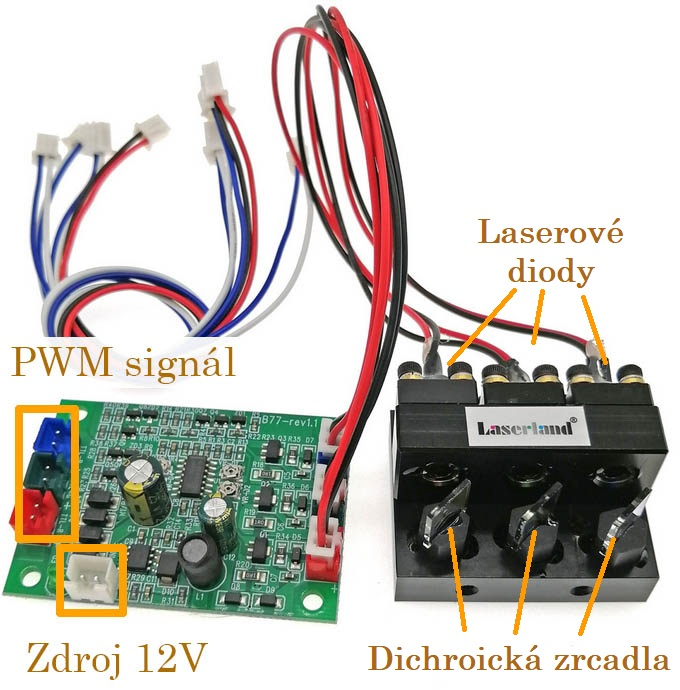
\includegraphics[width=0.8\textwidth]{img/hw_laser-module.jpg}
  \caption{\label{fig:hw_laser-module} Laserový modul s řídící deskou a vyznačenými konektory}
\end{figure}

\subsection{Dichroická zrcadla~\cite{dichroic-mirrors}}

Dichroická zrcadla jsou zrcadla s výrazně rodílnými odrazovými nebo průchodovými vlastnostmi pro dvě různé vlnové délky odraženého~/~procházejícího světla.

Většina dichroických zrcadel jsou dielektrická zrcádla -- zrcadla skládající se~z~mnoha tenkých vrstev různě opticky propustných materiálů, existují ale také krystalická zrcadla, jejiž odrážlivá vrstva se~skládá z~monokrystalického materiálu, typicky polovodiče.

Mezi jejich využití spadá například oddělování infračerveného záření při aplikacích, kdy je~nežádoucí zahřívání ozařovaného objektu.

\subsection{Zapojení laserového modulu}
K modulu je~od výroby připojená řídící deska. Ta~požaduje napětí 12~V a~přijímá binární signál pro každou diodu. Je-li na~signál připojen GND, korespondující dioda nesvítí. Je-li na~něj připojeno 2.7 až 5~V, korespondující dioda svítí.

\subsection{Tvorba barev s laserovým modulem}
S laserem je~tedy možné vytvořit 7 barev - červenou, zelenou, modrou, žlutou, tyrkysovou, purpurovou a~bílou, viz obrázek~\ref{fig:7colors}.

\begin{figure}[htb]
  \centering
  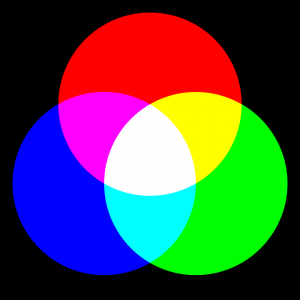
\includegraphics[width=0.3\textwidth]{img/7colors.png}
  \caption{\label{fig:7colors} Sedm základních barev laserového modulu}
\end{figure}

Naštěstí i~zde je~možné uplatnit jev persistance of~vision a~sice pomocí techniky PWM (z~anglického Pulse Width Modulation). Ta~se využívá jako alternativa analogového řízení v případech, kdy je~potřeba řídit analogovou proměnnou binárním signálem, tedy signálem nabývyjících hodnot \uv{zapnuto/vypnuto}.
V PWM signálu je~konstantní perioda a~proměnný je~čas, kdy má binární signál hodnotu \uv{zapnuto}, tomuto času se~říká \uv{pulse width} a~vyplývá z~něj jméno techniky. Konečná hodnota (\uv{střída}, anglicky \uv{duty cycle}) signálu se~dá získat jako poměr času \uv{pulse width} a~periody signálu. Střída hodnoty 100\% tedy znamená, že signál má neustále hodnotu \uv{zapnuto}, střída hodnoty 0\% naopak znamená neustálé \uv{vypnuto}.~\cite{pwm}\cite{wiki_pwm}

\begin{figure}[htb]
  \centering
  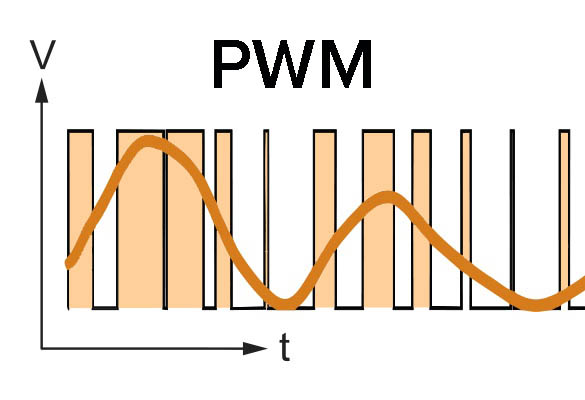
\includegraphics[width=0.4\textwidth]{img/pwm.jpg}
  \caption{\label{fig:pwm} PWM signál s měnící se střídou; Střída naznačena oranžovou křivkou. Převzato a~upraveno z~\cite{pwm-image}}
\end{figure}

Nastavíme-li tedy střídu signálu pro červenou diodu na~100\% a~pro zelenou diodu na~50\% výsledný paprsek bude pro lidské oko mít barvu s rgb hodnotou (255, 127, 0) neboli oranžovou.

I tato technologie má ovšem své limitace, řídící deska laserového modulu zvládá přijímat signál o maximální frekvenci 35~kHz (Raspberry Pi~je schopno vysílat s frekvencí až 40kHz), což vzhledem k rychlosti pohybu laseru v některých případech nemusí stačit.
Může se~stát, že při vykreslování křivky se~paprsek stihne posunout dříve, než uplyne perioda pwm signálu. Pokud se~tak stane budou různé sousední části křivky mít různou barvu.

\fxnote{TODO obrázek nedostatečně rychleho pwm}

Tento efekt je~nejviditelnější při projekci tmavých barev, ale dá se~zmírnit zvětšením času, po~který paprsek setrvá na~jednom bodě po~jeho vykreslení, v tu~chvíli se~ale může stát, že nastane \uv{flickering} popsaný v~sekci~\ref{sec:projection-princip}.